%%%%%%%%%%%%%%%%%%%%%%%%%%%%%%%%%%%%%%%%%
% All Presentation: Quantum Bayesian Game Theory
% Gabungan Teori dan Implementasi
%%%%%%%%%%%%%%%%%%%%%%%%%%%%%%%%%%%%%%%%%

\documentclass[aspectratio=169]{beamer}
\usepackage[utf8]{inputenc}
\usepackage{amsmath,amssymb,physics}
\usepackage{graphicx}
\usepackage{listings}
\usepackage{xcolor}
\usepackage{tikz}
\usepackage{booktabs}
\usepackage{hyperref}

% Theme
\usetheme{Madrid}
\usecolortheme{seahorse}

% Code listing style
\lstset{
    language=Python,
    basicstyle=\ttfamily\tiny,
    keywordstyle=\color{blue},
    stringstyle=\color{red},
    commentstyle=\color{gray},
    numbers=left,
    numberstyle=\tiny,
    numbersep=5pt,
    breaklines=true,
    showstringspaces=false,
    frame=single,
    backgroundcolor=\color{gray!10}
}

% Judul
\title{Quantum Bayesian Game Theory untuk Analisis Pasar}
\subtitle{Teori dan Implementasi}
\date{\today}

\begin{document}

% Slide Judul
\begin{frame}
    \titlepage
\end{frame}

%%%%%%%%%%%%%%%%%%%%%%%%%%%%%%%%%%%%%%%%%
%% BAGIAN I: TEORI
%%%%%%%%%%%%%%%%%%%%%%%%%%%%%%%%%%%%%%%%%

\part{Teori: Metodologi Quantum Bayesian Game Theory}
\frame{\partpage}

%%%%%%%%%%%%%%%%%%%%%%%%%%%%%%%%%%%%%%%%%
\section{Pendahuluan}
%%%%%%%%%%%%%%%%%%%%%%%%%%%%%%%%%%%%%%%%%

\begin{frame}{Pendahuluan}
    \begin{itemize}
        \item Metodologi yang menjembatani dinamika pasar (\textbf{Econophysics}) dengan interaksi strategis (\textbf{Game Theory})
        \item Menggunakan formalisme mekanika kuantum
        \item Menangkap ``keterikatan'' antar aset melalui probabilitas keadaan bersama
        \item Tidak sekadar korelasi linear, melainkan representasi \textbf{quantum state}
    \end{itemize}
\end{frame}

%%%%%%%%%%%%%%%%%%%%%%%%%%%%%%%%%%%%%%%%%
\section{Diagram Alur Metodologi}
%%%%%%%%%%%%%%%%%%%%%%%%%%%%%%%%%%%%%%%%%

\begin{frame}{Tahap A: Persiapan Data}
    \begin{columns}
        \begin{column}{0.55\textwidth}
            \begin{block}{Langkah-langkah:}
                \begin{enumerate}
                    \item \textbf{Input Data}: Data Keuangan Leader (Gold) \& Follower (Silver)
                    \item \textbf{Hitung Return}: Menggunakan \texttt{pct\_change()}
                    \item \textbf{Diskretisasi State}: Return $< 0 \Rightarrow$ State 1 (Turun)
                    \item \textbf{Looping \& Ekstraksi}: Menghasilkan $n_{ij}$ dan Sum Return
                \end{enumerate}
            \end{block}
            
            \vspace{0.3cm}
            \textbf{Output:}
            \begin{itemize}
                \item Variabel $n_{ij}$ (Frekuensi Kejadian)
                \item Variabel Sum Return (Total Return per State)
            \end{itemize}
        \end{column}
        \begin{column}{0.4\textwidth}
            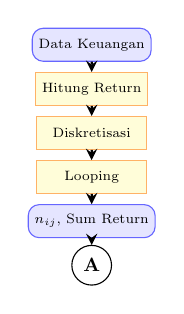
\begin{tikzpicture}[node distance=0.8cm, scale=0.7, transform shape]
                \tikzstyle{data} = [rectangle, rounded corners, minimum width=2cm, minimum height=0.6cm, text centered, draw=blue!60, fill=blue!10, font=\scriptsize]
                \tikzstyle{process} = [rectangle, minimum width=2cm, minimum height=0.6cm, text centered, draw=orange!60, fill=yellow!15, font=\scriptsize]
                \tikzstyle{arrow} = [thick,->,>=stealth]
                
                \node (input) [data] {Data Keuangan};
                \node (return) [process, below of=input] {Hitung Return};
                \node (disc) [process, below of=return] {Diskretisasi};
                \node (loop) [process, below of=disc] {Looping};
                \node (nij) [data, below of=loop] {$n_{ij}$, Sum Return};
                \node (conn) [circle, draw, below of=nij, minimum size=0.5cm] {\textbf{A}};
                
                \draw [arrow] (input) -- (return);
                \draw [arrow] (return) -- (disc);
                \draw [arrow] (disc) -- (loop);
                \draw [arrow] (loop) -- (nij);
                \draw [arrow] (nij) -- (conn);
            \end{tikzpicture}
        \end{column}
    \end{columns}
\end{frame}

\begin{frame}{Tahap B: Matriks Payoff Game Theory}
    \begin{columns}
        \begin{column}{0.55\textwidth}
            \begin{block}{Langkah-langkah:}
                \begin{enumerate}
                    \item \textbf{Input}: Dari \textbf{(A)} $n_{ij}$ dan Sum Return
                    \item \textbf{Rumus Payoff}: $\text{Payoff} = \frac{\text{Sum}}{n + 1}$
                    \item \textbf{Hitung Selisih}: Payoff Naik $-$ Payoff Turun
                \end{enumerate}
            \end{block}
            
            \vspace{0.3cm}
            \textbf{Output:}
            \begin{itemize}
                \item Payoff Leader $(a, c, e, g)$
                \item Payoff Follower $(b, d, f, h)$
                \item Parameter Bias $h_L, h_F$
            \end{itemize}
        \end{column}
        \begin{column}{0.4\textwidth}
            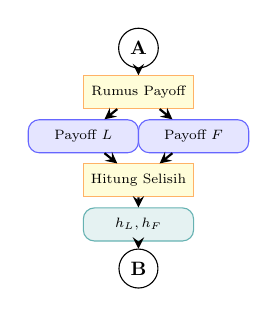
\begin{tikzpicture}[node distance=0.8cm, scale=0.7, transform shape]
                \tikzstyle{data} = [rectangle, rounded corners, minimum width=2cm, minimum height=0.6cm, text centered, draw=blue!60, fill=blue!10, font=\scriptsize]
                \tikzstyle{process} = [rectangle, minimum width=2cm, minimum height=0.6cm, text centered, draw=orange!60, fill=yellow!15, font=\scriptsize]
                \tikzstyle{param} = [rectangle, rounded corners, minimum width=2cm, minimum height=0.6cm, text centered, draw=teal!60, fill=teal!10, font=\scriptsize]
                \tikzstyle{arrow} = [thick,->,>=stealth]
                
                \node (connA) [circle, draw, minimum size=0.5cm] {\textbf{A}};
                \node (payoff) [process, below of=connA] {Rumus Payoff};
                \node (pL) [data, below of=payoff, xshift=-1cm] {Payoff $L$};
                \node (pF) [data, below of=payoff, xshift=1cm] {Payoff $F$};
                \node (bias) [process, below of=pL, xshift=1cm] {Hitung Selisih};
                \node (h) [param, below of=bias] {$h_L, h_F$};
                \node (connB) [circle, draw, below of=h, minimum size=0.5cm] {\textbf{B}};
                
                \draw [arrow] (connA) -- (payoff);
                \draw [arrow] (payoff) -- (pL);
                \draw [arrow] (payoff) -- (pF);
                \draw [arrow] (pL) -- (bias);
                \draw [arrow] (pF) -- (bias);
                \draw [arrow] (bias) -- (h);
                \draw [arrow] (h) -- (connB);
            \end{tikzpicture}
        \end{column}
    \end{columns}
\end{frame}

\begin{frame}{Tahap C: Probabilitas \& Entanglement}
    \begin{columns}
        \begin{column}{0.55\textwidth}
            \begin{block}{Langkah-langkah:}
                \begin{enumerate}
                    \item \textbf{Input}: Dari \textbf{(A)} $n_{ij}$
                    \item \textbf{Normalisasi}: $P_{ij} = n_{ij} / n_{total}$
                    \item \textbf{Amplitudo}: $a_{ij} = \sqrt{P_{ij}}$
                    \item \textbf{Density Matrix}: $\rho = \ket{\psi}\bra{\psi}$
                    \item \textbf{Partial Trace}: $\rho_L, \rho_F$
                    \item \textbf{Von Neumann Entropy}: $S = -\text{Tr}(\rho \ln \rho)$
                    \item \textbf{QMI}: $I = S_L + S_F - S_{LF}$
                \end{enumerate}
            \end{block}
            
            \textbf{Output:} Parameter Interaksi $J_{LF}$
        \end{column}
        \begin{column}{0.4\textwidth}
            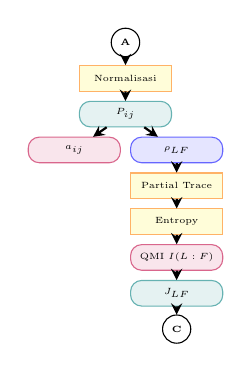
\begin{tikzpicture}[node distance=0.7cm, scale=0.65, transform shape]
                \tikzstyle{data} = [rectangle, rounded corners, minimum width=1.8cm, minimum height=0.5cm, text centered, draw=blue!60, fill=blue!10, font=\tiny]
                \tikzstyle{process} = [rectangle, minimum width=1.8cm, minimum height=0.5cm, text centered, draw=orange!60, fill=yellow!15, font=\tiny]
                \tikzstyle{param} = [rectangle, rounded corners, minimum width=1.8cm, minimum height=0.5cm, text centered, draw=teal!60, fill=teal!10, font=\tiny]
                \tikzstyle{result} = [rectangle, rounded corners, minimum width=1.8cm, minimum height=0.5cm, text centered, draw=purple!60, fill=purple!10, font=\tiny]
                \tikzstyle{arrow} = [thick,->,>=stealth]
                
                \node (connA) [circle, draw, minimum size=0.4cm, font=\tiny] {\textbf{A}};
                \node (norm) [process, below of=connA] {Normalisasi};
                \node (prob) [param, below of=norm] {$P_{ij}$};
                \node (amp) [result, below of=prob, xshift=-1cm] {$a_{ij}$};
                \node (rho) [data, below of=prob, xshift=1cm] {$\rho_{LF}$};
                \node (trace) [process, below of=rho] {Partial Trace};
                \node (entropy) [process, below of=trace] {Entropy};
                \node (qmi) [result, below of=entropy] {QMI $I(L:F)$};
                \node (j) [param, below of=qmi] {$J_{LF}$};
                \node (connC) [circle, draw, below of=j, minimum size=0.4cm, font=\tiny] {\textbf{C}};
                
                \draw [arrow] (connA) -- (norm);
                \draw [arrow] (norm) -- (prob);
                \draw [arrow] (prob) -- (amp);
                \draw [arrow] (prob) -- (rho);
                \draw [arrow] (rho) -- (trace);
                \draw [arrow] (trace) -- (entropy);
                \draw [arrow] (entropy) -- (qmi);
                \draw [arrow] (qmi) -- (j);
                \draw [arrow] (j) -- (connC);
            \end{tikzpicture}
        \end{column}
    \end{columns}
\end{frame}

\begin{frame}{Tahap D: Model Hamiltonian}
    \begin{columns}
        \begin{column}{0.55\textwidth}
            \begin{block}{Langkah-langkah:}
                \begin{enumerate}
                    \item \textbf{Input}: Dari \textbf{(B)} $h_L, h_F$ dan \textbf{(C)} $J_{LF}$
                    \item \textbf{Konstruksi Hamiltonian}: 
                    $$H = -\sum h_i \sigma_i^z - J(\sigma_L^z \sigma_F^z)$$
                    \item \textbf{Eigendecomposition}: Mencari eigenvalues
                \end{enumerate}
            \end{block}
            
            \vspace{0.3cm}
            \textbf{Output:}
            \begin{itemize}
                \item Matriks Hamiltonian $H$
                \item Ground State Energy
                \item Vektor Keadaan Paling Stabil
            \end{itemize}
        \end{column}
        \begin{column}{0.4\textwidth}
            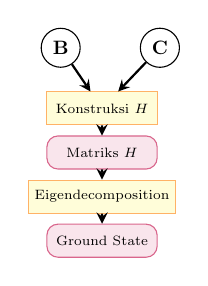
\begin{tikzpicture}[node distance=0.8cm, scale=0.7, transform shape]
                \tikzstyle{process} = [rectangle, minimum width=2cm, minimum height=0.6cm, text centered, draw=orange!60, fill=yellow!15, font=\scriptsize]
                \tikzstyle{result} = [rectangle, rounded corners, minimum width=2cm, minimum height=0.6cm, text centered, draw=purple!60, fill=purple!10, font=\scriptsize]
                \tikzstyle{arrow} = [thick,->,>=stealth]
                
                \node (connB) [circle, draw, minimum size=0.5cm] {\textbf{B}};
                \node (connC) [circle, draw, right of=connB, xshift=1cm, minimum size=0.5cm] {\textbf{C}};
                \node (const) [process, below of=connB, xshift=0.75cm, yshift=-0.3cm] {Konstruksi $H$};
                \node (H) [result, below of=const] {Matriks $H$};
                \node (eigen) [process, below of=H] {Eigendecomposition};
                \node (ground) [result, below of=eigen] {Ground State};
                
                \draw [arrow] (connB) -- (const);
                \draw [arrow] (connC) -- (const);
                \draw [arrow] (const) -- (H);
                \draw [arrow] (H) -- (eigen);
                \draw [arrow] (eigen) -- (ground);
            \end{tikzpicture}
        \end{column}
    \end{columns}
\end{frame}

%%%%%%%%%%%%%%%%%%%%%%%%%%%%%%%%%%%%%%%%%
\section{Konstruksi Matriks Payoff}
%%%%%%%%%%%%%%%%%%%%%%%%%%%%%%%%%%%%%%%%%

\begin{frame}{Skema Leader-Follower (Stackelberg)}
    \begin{itemize}
        \item Pergerakan harga diperlakukan sebagai strategi
        \item Notasi bra-ket $\ket{\cdot}$ untuk merepresentasikan \textit{state} diskrit (naik/turun)
    \end{itemize}
    
    \vspace{0.5cm}
    
    \begin{table}
        \centering
        \begin{tabular}{c|c|c}
            \toprule
            \textbf{Leader / Follower} & $\ket{0}_F$ (Up) & $\ket{1}_F$ (Down) \\
            \midrule
            $\ket{0}_L$ (Up) & $(a, b)$ & $(c, d)$ \\
            $\ket{1}_L$ (Down) & $(e, f)$ & $(g, h)$ \\
            \bottomrule
        \end{tabular}
    \end{table}
\end{frame}

\begin{frame}{Rumus Nilai Payoff}
    Nilai payoff dihitung menggunakan rata-rata return dengan Laplace smoothing:
    
    \begin{align}
        a &= \frac{\sum L^{00}}{n_{00} + 1}, \quad b = \frac{\sum F^{00}}{n_{00} + 1} \\[10pt]
        c &= \frac{\sum L^{01}}{n_{01} + 1}, \quad d = \frac{\sum F^{01}}{n_{01} + 1} \\[10pt]
        e &= \frac{\sum L^{10}}{n_{10} + 1}, \quad f = \frac{\sum F^{10}}{n_{10} + 1} \\[10pt]
        g &= \frac{\sum L^{11}}{n_{11} + 1}, \quad h = \frac{\sum F^{11}}{n_{11} + 1}
    \end{align}
    
    \vspace{0.3cm}
    Dimana $n_{ij}$ adalah jumlah kejadian state $(i,j)$
\end{frame}

%%%%%%%%%%%%%%%%%%%%%%%%%%%%%%%%%%%%%%%%%
\section{Pemodelan Game Theory}
%%%%%%%%%%%%%%%%%%%%%%%%%%%%%%%%%%%%%%%%%

\begin{frame}{Klasifikasi Tipe Permainan}
    Berdasarkan nilai payoff, hubungan antar aset dapat diklasifikasikan:
    
    \begin{itemize}
        \item \textbf{Coordination Game}: Payoff tertinggi pada $(0,0)$ dan $(1,1)$
            \begin{itemize}
                \item Aset bergerak searah (korelasi positif kuat)
            \end{itemize}
        \item \textbf{Anti-Coordination}: Payoff tertinggi pada $(0,1)$ atau $(1,0)$
            \begin{itemize}
                \item Hubungan substitusi atau \textit{hedging}
            \end{itemize}
        \item \textbf{Prisoner's Dilemma}: Ada insentif ``mengkhianati'' arah tren
    \end{itemize}
    
    \vspace{0.5cm}
    \textbf{Nash Equilibrium}: Jika $a > e$ dan $b > d$, maka $\ket{00}$ adalah equilibrium
\end{frame}

\begin{frame}{Bayesian Game}
    \begin{itemize}
        \item Matriks dapat menjadi \textbf{Bayesian Game}
        \item \textbf{Type}: Kondisi internal pasar (bullish/bearish tersembunyi)
        \item \textbf{Beliefs}: Probabilitas pergerakan lawan
    \end{itemize}
    
    \vspace{0.5cm}
    
    Keadaan $\ket{\psi}$ merepresentasikan \textit{Joint Probability Distribution} yang mendasari \textbf{Bayesian Nash Equilibrium}
\end{frame}

%%%%%%%%%%%%%%%%%%%%%%%%%%%%%%%%%%%%%%%%%
\section{Quantum Entanglement}
%%%%%%%%%%%%%%%%%%%%%%%%%%%%%%%%%%%%%%%%%

\begin{frame}{Konstruksi Quantum State}
    Sistem dua aset direpresentasikan sebagai fungsi gelombang:
    
    \begin{equation}
        \ket{\psi} = a_{00} \ket{00} + a_{01} \ket{01} + a_{10} \ket{10} + a_{11} \ket{11}
    \end{equation}
    
    \vspace{0.5cm}
    
    \begin{itemize}
        \item $|a_{ij}|^2 = P(\ket{ij})$ adalah probabilitas gabungan
        \item Koefisien dihitung dari: $a_{ij} = \sqrt{P_{ij}}$
    \end{itemize}
\end{frame}

\begin{frame}{Reduced Density Matrix \& Entanglement}
    Untuk mengukur derajat ketergantungan (entanglement):
    
    \begin{enumerate}
        \item Bentuk matriks densitas: $\rho = \ket{\psi}\bra{\psi}$
        \item Partial trace: $\rho_L = \text{Tr}_F(\rho)$
        \item Von Neumann Entropy:
        \begin{equation}
            S = -\text{Tr}(\rho_L \ln \rho_L)
        \end{equation}
    \end{enumerate}
    
    \vspace{0.5cm}
    
    \textbf{Interpretasi}: Jika $S > 0$, kedua aset \textit{ter-entangle} secara informasi
\end{frame}

\begin{frame}{Quantum Mutual Information}
    \begin{equation}
        I(L:F) = S(\rho_L) + S(\rho_F) - S(\rho_{LF})
    \end{equation}
    
    \vspace{0.5cm}
    
    \begin{itemize}
        \item Semakin tinggi nilai $I$, semakin kuat keterikatan
        \item Menunjukkan ``kluster kuantum'' di pasar keuangan
        \item Aset bergerak sebagai satu kesatuan fungsi gelombang
    \end{itemize}
\end{frame}

%%%%%%%%%%%%%%%%%%%%%%%%%%%%%%%%%%%%%%%%%
\section{Network Theory}
%%%%%%%%%%%%%%%%%%%%%%%%%%%%%%%%%%%%%%%%%

\begin{frame}{Quantum Financial Network}
    Untuk lebih dari 2 aset:
    
    \begin{itemize}
        \item \textbf{Nodes}: Setiap aset
        \item \textbf{Edges}: Nilai Entanglement Entropy atau Quantum Mutual Information
    \end{itemize}
    
    \vspace{0.5cm}
    
    Metode ini memungkinkan:
    \begin{itemize}
        \item Melihat siapa yang berkorelasi dengan siapa
        \item Menemukan ``penggerak utama'' (Leader) menggunakan \textbf{Eigenvector Centrality}
    \end{itemize}
\end{frame}

%%%%%%%%%%%%%%%%%%%%%%%%%%%%%%%%%%%%%%%%%
\section{Konstruksi Hamiltonian}
%%%%%%%%%%%%%%%%%%%%%%%%%%%%%%%%%%%%%%%%%

\begin{frame}{Model Ising Hamiltonian}
    Hamiltonian merepresentasikan \textbf{total energi} atau \textbf{fungsi biaya} sistem:
    
    \begin{equation}
        H = -\sum h_i \sigma_i^z - \sum J_{ij} \sigma_i^z \sigma_j^z
    \end{equation}
    
    \vspace{0.3cm}
    
    Komponen:
    \begin{itemize}
        \item \textbf{Field Term}: $H_{bias} = -\sum_{i} h_i \sigma_i^z$
            \begin{itemize}
                \item $h_i$ dari selisih payoff naik vs turun
            \end{itemize}
        \item \textbf{Interaction Term}: $H_{int} = -J_{LF} (\sigma_L^z \sigma_F^z)$
            \begin{itemize}
                \item $J_{LF} > 0$: Coordination Game (Feromagnetik)
                \item $J_{LF} < 0$: Anti-coordination
            \end{itemize}
    \end{itemize}
\end{frame}

\begin{frame}{Pemetaan Parameter}
    Menentukan bias ($h$) dari payoff:
    \begin{equation}
        h_L = \frac{1}{2}\left[(a+c) - (e+g)\right], \quad h_F = \frac{1}{2}\left[(b+f) - (d+h)\right]
    \end{equation}
    
    \vspace{0.3cm}
    
    Menentukan interaksi ($J$) dari Quantum Mutual Information:
    \begin{equation}
        J_{LF} = \text{sgn}(\rho_{LF}) \cdot I(L:F)
    \end{equation}
    
    \small
    Dimana:
    \begin{itemize}
        \item $\text{sgn}(\rho_{LF})$: Tanda korelasi antar aset ($+1$ jika positif, $-1$ jika negatif)
        \item $I(L:F)$: Quantum Mutual Information
    \end{itemize}
\end{frame}

%%%%%%%%%%%%%%%%%%%%%%%%%%%%%%%%%%%%%%%%%
%% BAGIAN II: IMPLEMENTASI
%%%%%%%%%%%%%%%%%%%%%%%%%%%%%%%%%%%%%%%%%

\part{Implementasi: Kode Python}
\frame{\partpage}

%%%%%%%%%%%%%%%%%%%%%%%%%%%%%%%%%%%%%%%%%
\section{Import Library dan Data}
%%%%%%%%%%%%%%%%%%%%%%%%%%%%%%%%%%%%%%%%%

\begin{frame}[fragile]{Import Library}
\begin{lstlisting}
import yfinance as yf
import numpy as np
import pandas as pd
import scipy.linalg as la
import networkx as nx
import matplotlib.pyplot as plt
\end{lstlisting}

\vspace{0.3cm}
Library yang digunakan:
\begin{itemize}
    \item \texttt{yfinance}: Mengambil data historis aset
    \item \texttt{numpy}, \texttt{scipy}: Komputasi numerik dan aljabar linear
    \item \texttt{networkx}: Analisis jaringan
\end{itemize}
\end{frame}

\begin{frame}[fragile]{Fungsi Pengambilan Data}
\begin{lstlisting}
def get_market_data(tickers, period="2y"):
    data = yf.download(tickers, period=period)['Close']
    returns = data.pct_change().dropna()
    return returns

# Eksekusi
tickers = ['GC=F', 'SI=F']  # Gold dan Silver
data_returns = get_market_data(tickers)
\end{lstlisting}
\end{frame}

%%%%%%%%%%%%%%%%%%%%%%%%%%%%%%%%%%%%%%%%%
\section{Konstruksi Matriks Payoff (Kode)}
%%%%%%%%%%%%%%%%%%%%%%%%%%%%%%%%%%%%%%%%%

\begin{frame}[fragile]{Fungsi Analisis Quantum Game}
\begin{lstlisting}
def analyze_quantum_game(returns, leader_col, follower_col):
    # Tentukan state: 0 jika naik (up), 1 jika turun (down)
    L_state = (returns[leader_col] < 0).astype(int)
    F_state = (returns[follower_col] < 0).astype(int)
    
    # Inisialisasi frekuensi dan akumulasi return
    n_ij = np.zeros((2, 2))
    sum_L = np.zeros((2, 2))
    sum_F = np.zeros((2, 2))
    
    for i in range(len(returns)):
        l, f = L_state.iloc[i], F_state.iloc[i]
        n_ij[l, f] += 1
        sum_L[l, f] += returns[leader_col].iloc[i]
        sum_F[l, f] += returns[follower_col].iloc[i]
\end{lstlisting}
\end{frame}

\begin{frame}[fragile]{Perhitungan Payoff dan Amplitudo}
\begin{lstlisting}
    n_total = n_ij.sum()
    
    # Nilai payoff dengan Laplace Smoothing
    payoff_L = sum_L / (n_ij + 1)
    payoff_F = sum_F / (n_ij + 1)
    
    # Quantum State Coefficients (Amplitudo Probabilitas)
    prob_matrix = n_ij / n_total
    amplitudes = np.sqrt(prob_matrix)  # a00, a01, a10, a11
    
    return payoff_L, payoff_F, amplitudes, prob_matrix
\end{lstlisting}
\end{frame}

\begin{frame}{Hasil Matriks Payoff}
    Output dari analisis Emas (GC=F) vs Perak (SI=F):
    
    \vspace{0.3cm}
    
    \textbf{Matriks Payoff Leader (Gold):}
    \begin{equation*}
        \begin{bmatrix} 0.0104 & 0.0045 \\ -0.0044 & -0.0107 \end{bmatrix}
    \end{equation*}
    
    \textbf{Matriks Payoff Follower (Silver):}
    \begin{equation*}
        \begin{bmatrix} 0.0204 & -0.0085 \\ 0.0071 & -0.0212 \end{bmatrix}
    \end{equation*}
    
    \textbf{Quantum State Coefficients:}
    \begin{equation*}
        \begin{bmatrix} 0.684 & 0.357 \\ 0.334 & 0.541 \end{bmatrix}
    \end{equation*}
\end{frame}

%%%%%%%%%%%%%%%%%%%%%%%%%%%%%%%%%%%%%%%%%
\section{Perhitungan Entropi Kuantum (Kode)}
%%%%%%%%%%%%%%%%%%%%%%%%%%%%%%%%%%%%%%%%%

\begin{frame}[fragile]{Konstruksi Matriks Densitas}
\begin{lstlisting}
# Matriks Densitas Global
rho_LF = probs / np.sum(probs) 

# Reduced Density Matrix untuk Leader (trace out Follower)
rho_L = np.diag([probs[0,0] + probs[0,1], probs[1,0] + probs[1,1]])

# Reduced Density Matrix untuk Follower (trace out Leader)
rho_F = np.diag([probs[0,0] + probs[1,0], probs[0,1] + probs[1,1]])
\end{lstlisting}
\end{frame}

\begin{frame}[fragile]{Fungsi Von Neumann Entropy}
\begin{lstlisting}
def von_neumann_entropy(rho):
    """Menghitung entropi S = -Tr(rho * log2(rho))"""
    eigvals = la.eigvalsh(rho)
    eigvals = eigvals[eigvals > 1e-12]
    return -np.sum(eigvals * np.log2(eigvals))

# Hitung Entropi
s_L = von_neumann_entropy(rho_L)
s_F = von_neumann_entropy(rho_F)
s_LF = von_neumann_entropy(rho_LF)

# Quantum Mutual Information
qmi = s_L + s_F - s_LF
\end{lstlisting}
\end{frame}

\begin{frame}{Hasil Analisis Entropi}
    \begin{table}
        \centering
        \begin{tabular}{lc}
            \toprule
            \textbf{Metrik} & \textbf{Nilai} \\
            \midrule
            Entropi Emas ($S_L$) & 0.9735 \\
            Entropi Perak ($S_F$) & 0.9816 \\
            Quantum Mutual Information ($I$) & 0.9724 \\
            \bottomrule
        \end{tabular}
    \end{table}
    
    \vspace{0.5cm}
    
    \textbf{Interpretasi}: Entanglement sangat kuat. Emas dan Perak memiliki ``jalur informasi'' yang hampir identik.
\end{frame}

%%%%%%%%%%%%%%%%%%%%%%%%%%%%%%%%%%%%%%%%%
\section{Analisis Network Theory (Kode)}
%%%%%%%%%%%%%%%%%%%%%%%%%%%%%%%%%%%%%%%%%

\begin{frame}[fragile]{Membangun Quantum Financial Network}
\begin{lstlisting}
# Definisikan daftar aset
tickers_list = ['GC=F', 'SI=F', 'CL=F', 'HG=F', 'BTC-USD', 'AAPL']

# Bangun Matriks Adjasensi berdasarkan QMI
G = nx.Graph()

for i, a in enumerate(tickers_list):
    for j, b in enumerate(tickers_list):
        if i < j:
            qmi_val = calculate_qmi_pair(all_data, a, b)
            G.add_edge(a, b, weight=qmi_val)
\end{lstlisting}
\end{frame}

\begin{frame}{Visualisasi Quantum Financial Network}
    \begin{columns}
        \begin{column}{0.45\textwidth}
            \begin{center}
                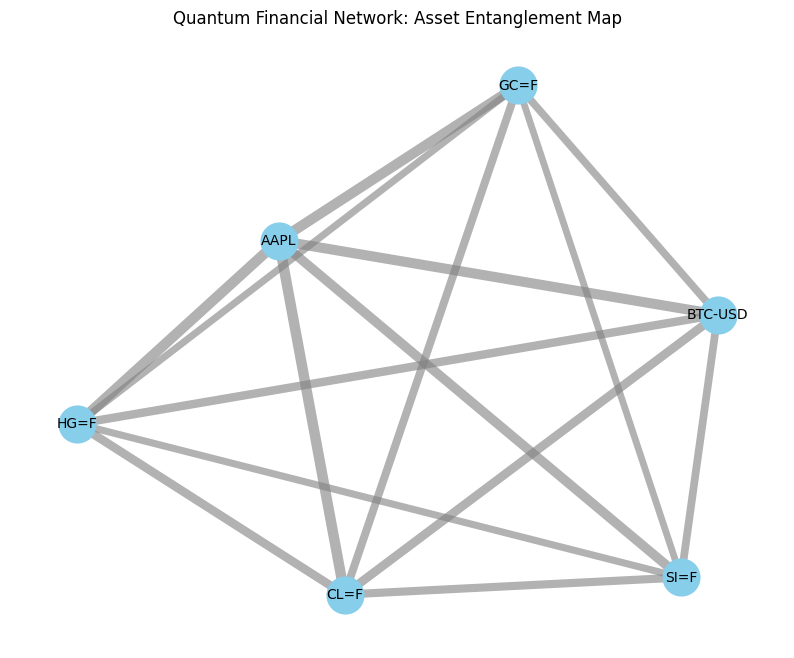
\includegraphics[width=\textwidth]{Network.png}
            \end{center}
        \end{column}
        \begin{column}{0.52\textwidth}
            \small
            \textbf{Komponen Graf:}
            \begin{itemize}
                \item \textbf{Node}: Aset keuangan
                \item \textbf{Edge}: Kekuatan QMI antar aset
            \end{itemize}
            
            \vspace{0.3cm}
            \textbf{Interpretasi:}
            \begin{itemize}
                \item Garis tebal $\Rightarrow$ entanglement kuat
                \item HG=F (Copper) memiliki banyak koneksi kuat
                \item GC=F \& SI=F (Gold-Silver) terhubung erat
                \item BTC-USD relatif terpisah dari komoditas
                \item AAPL berperan sebagai ``bridge'' antar kluster
            \end{itemize}
        \end{column}
    \end{columns}
\end{frame}

\begin{frame}[fragile]{Eigenvector Centrality Analysis}
\begin{lstlisting}
# Cari Leader Utama dengan Eigenvector Centrality
centrality = nx.eigenvector_centrality(G, weight='weight')
sorted_centrality = sorted(centrality.items(), 
                           key=lambda x: x[1], reverse=True)
\end{lstlisting}

\vspace{0.3cm}

\textbf{Hasil Centrality Analysis (Market Leaders):}
\begin{table}
    \centering
    \begin{tabular}{lc}
        \toprule
        \textbf{Asset} & \textbf{Centrality} \\
        \midrule
        AAPL & 0.4642 \\
        CL=F & 0.4158 \\
        BTC-USD & 0.4054 \\
        HG=F & 0.3980 \\
        GC=F & 0.3812 \\
        SI=F & 0.3789 \\
        \bottomrule
    \end{tabular}
\end{table}
\end{frame}

%%%%%%%%%%%%%%%%%%%%%%%%%%%%%%%%%%%%%%%%%
\section{Konstruksi Hamiltonian (Kode)}
%%%%%%%%%%%%%%%%%%%%%%%%%%%%%%%%%%%%%%%%%

\begin{frame}[fragile]{Perhitungan Parameter Hamiltonian}
\begin{lstlisting}
# 1. Hitung parameter bias (h) dan interaksi (J)
h_L = (pL[0,0] + pL[0,1]) - (pL[1,0] + pL[1,1])
h_F = (pF[0,0] + pF[1,0]) - (pF[0,1] + pF[1,1])
J_LF = qmi  # Quantum Mutual Information sebagai kekuatan interaksi

# 2. Definisikan Operator Pauli-Z dan Identitas
Z = np.array([[1, 0], [0, -1]])
I_mat = np.eye(2)
\end{lstlisting}
\end{frame}

\begin{frame}[fragile]{Konstruksi Matriks Hamiltonian}
\begin{lstlisting}
# 3. Konstruksi Hamiltonian menggunakan Tensor Product
# H = -hL(Z x I) - hF(I x Z) - J(Z x Z)
H = -h_L * np.kron(Z, I_mat) - h_F * np.kron(I_mat, Z) \
    - J_LF * np.kron(Z, Z)

# 4. Mencari Ground State (Energi Terendah)
eigenvalues, eigenvectors = la.eigh(H)
ground_state_energy = eigenvalues[0]
ground_state_vector = eigenvectors[:, 0]
\end{lstlisting}
\end{frame}

\begin{frame}{Hasil Matriks Hamiltonian}
    \textbf{Matriks Hamiltonian Sistem (4x4):}
    \begin{equation*}
        H = \begin{bmatrix}
            -1.0596 & 0 & 0 & 0 \\
            0 & 0.9997 & 0 & 0 \\
            0 & 0 & 0.9451 & 0 \\
            0 & 0 & 0 & -0.8852
        \end{bmatrix}
    \end{equation*}
    
    \vspace{0.3cm}
    
    \begin{itemize}
        \item \textbf{Energi Ground State}: $-1.0596$
        \item \textbf{Vektor Keadaan Paling Stabil}: $[1, 0, 0, 0]$ (keadaan $\ket{00}$)
    \end{itemize}
\end{frame}

\end{document}
